%Style
\documentclass[12pt]{article}
\usepackage[top=1in, bottom=1in, left=1in, right=1in]{geometry}
\parindent 22pt
\usepackage{fancyhdr}

%Packages
\usepackage{adjustbox}
\usepackage{amsmath}
\usepackage{amsfonts}
\usepackage{amssymb}
\usepackage{bm}
\usepackage[table]{xcolor}
\usepackage{tabu}
\usepackage{makecell}
\usepackage{longtable}
\usepackage{multirow}
\usepackage[normalem]{ulem}
\usepackage{etoolbox}
\usepackage{graphicx}
\usepackage{tabularx}
\usepackage{ragged2e}
\usepackage{booktabs}
\usepackage{caption}
\usepackage{fixltx2e}
\usepackage[para, flushleft]{threeparttablex}
\usepackage[capposition=top]{floatrow}
\usepackage{subcaption}
\usepackage{pdfpages}
\usepackage{pdflscape}
\usepackage{natbib}
\usepackage{bibunits}
\definecolor{maroon}{HTML}{990012}
\usepackage[colorlinks=true,linkcolor=maroon,citecolor=maroon,urlcolor=maroon,anchorcolor=maroon]{hyperref}
\usepackage{marvosym}
\usepackage{makeidx}
\usepackage{tikz}
\usetikzlibrary{shapes}
\usepackage{setspace}
\usepackage{enumerate}
\usepackage{rotating}
\usepackage{epstopdf}
\usepackage[titletoc]{appendix}
\usepackage{framed}
\usepackage{comment}
\usepackage{xr}
\usepackage{titlesec}
\usepackage{footnote}
\usepackage{longtable}
\newlength{\tablewidth}
\setlength{\tablewidth}{9.3in}
\setcounter{secnumdepth}{4}

\titleformat{\paragraph}
{\normalfont\normalsize\bfseries}{\theparagraph}{1em}{}
\titlespacing*{\paragraph}
{0pt}{3.25ex plus 1ex minus .2ex}{1.5ex plus .2ex}
\makeatletter
\pretocmd\start@align
{%
  \let\everycr\CT@everycr
  \CT@start
}{}{}
\apptocmd{\endalign}{\CT@end}{}{}
\makeatother
%Watermark
\usepackage[printwatermark]{xwatermark}
\usepackage{lipsum}
\definecolor{lightgray}{RGB}{220,220,220}
%\newwatermark[allpages,color=lightgray,angle=45,scale=3,xpos=0,ypos=0]{Preliminary Draft}

%Further subsection level
\usepackage{titlesec}
\setcounter{secnumdepth}{4}
\titleformat{\paragraph}
{\normalfont\normalsize\bfseries}{\theparagraph}{1em}{}
\titlespacing*{\paragraph}
{0pt}{3.25ex plus 1ex minus .2ex}{1.5ex plus .2ex}

\setcounter{secnumdepth}{5}
\titleformat{\subparagraph}
{\normalfont\normalsize\bfseries}{\thesubparagraph}{1em}{}
\titlespacing*{\subparagraph}
{0pt}{3.25ex plus 1ex minus .2ex}{1.5ex plus .2ex}

%Functions
\DeclareMathOperator{\cov}{Cov}
\DeclareMathOperator{\var}{Var}
\DeclareMathOperator{\plim}{plim}
\DeclareMathOperator*{\argmin}{arg\,min}
\DeclareMathOperator*{\argmax}{arg\,max}

%Math Environments
\newtheorem{theorem}{Theorem}[section]
\newtheorem{claim}[theorem]{Claim}
\newtheorem{assumption}[theorem]{Assumption}
\newtheorem{definition}[theorem]{Definition}
\newtheorem{hypothesis}[theorem]{Hypothesis}
\newtheorem{property}[theorem]{Property}
\newtheorem{example}[theorem]{Example}
\newtheorem{condition}[theorem]{Condition}
\newtheorem{result}[theorem]{Result}
\newenvironment{proof}{\paragraph{Proof:}}{\hfill$\square$}

%Commands
\newcommand\independent{\protect\mathpalette{\protect\independenT}{\perp}}
\def\independenT#1#2{\mathrel{\rlap{$#1#2$}\mkern2mu{#1#2}}}
\newcommand{\overbar}[1]{\mkern 1.5mu\overline{\mkern-1.5mu#1\mkern-1.5mu}\mkern 1.5mu}
\newcommand{\equald}{\ensuremath{\overset{d}{=}}}
\captionsetup[table]{skip=10pt}
%\makeindex


\newcolumntype{L}[1]{>{\raggedright\let\newline\\\arraybackslash\hspace{0pt}}m{#1}}
\newcolumntype{C}[1]{>{\centering\let\newline\\\arraybackslash\hspace{0pt}}m{#1}}
\newcolumntype{R}[1]{>{\raggedleft\let\newline\\\arraybackslash\hspace{0pt}}m{#1}}



%Logo
%\AddToShipoutPictureBG{%
%  \AtPageUpperLeft{\raisebox{-\height}{\includegraphics[width=1.5cm]{uchicago.png}}}
%}

\newcolumntype{L}[1]{>{\raggedright\let\newline\\\arraybackslash\hspace{0pt}}m{#1}}
\newcolumntype{C}[1]{>{\centering\let\newline\\\arraybackslash\hspace{0pt}}m{#1}}
\newcolumntype{R}[1]{>{\raggedleft\let\newline\\\arraybackslash\hspace{0pt}}m{#1}} 

\newcommand{\mr}{\multirow}
\newcommand{\mc}{\multicolumn}

%\newcommand{\comment}[1]{}



\begin{document}

\title{Self-Reported Childcare Attendance Information in the Reggio Data}
\author{Reggio Team}
\date{Original version: Thursday 8\textsuperscript{th} September, 2016 \\ Current version: \today}
\maketitle

\doublespacing

\section{Introduction}

This report explores the possible issues regarding self-reported childcare attendance information in the Reggio data. How we categorize the types of childcare centers attended is following: 
\begin{enumerate}
\item Subjects (for adult cohorts) or mothers (for younger cohorts) answer survey questions that ask for school name, school type, and school street address of the preschool that they/their children attended. 
\item Based on the information provided by the respondents, we check if all information provided match with the actual childcare center information. If there are mismatches, we re-assign the childcare centers that they have more likely gone to.
\item If the responses are missing for some questions, we assign the childcare centers that the respondents/children have likely gone to based on the non-missing information. 
\item We generate the ``accuracy rate" on the childcare attendance information based on missing response problem and information mismatch problem. 
\end{enumerate}

However, there are some possibilities that some of our current school information in the data might have errors. This report compares the school information with the historical facts and better understand the possible data problems existing in the data. 

Table \ref{tab:cohort-structure} shows the existing age cohorts in the data, their years of birth, and the age at interview. Figure \ref{fig:attended-itc} and \ref{fig:attended-preschool} show the type of infant-toddler centers and preschools, respectively, attended by the subjects in the data. All the information is crucial to determine if the school information in our data matches with historical facts regarding the evolution of childcare in the Northern Italy.

\begin{table}[H] \caption{Cohort Structure} \label{tab:cohort-structure}
\begin{tabular}{ccc}
\toprule
Cohort & Years of Birth & Age at Interview \\ \midrule
I 	   & 1954-1959 		& 54-60 \\
II 	   & 1969-1970		& 43	\\
III    & 1980-1981		& 32    \\
IV 	   & 1994			& 18 	\\
V 	   & 2006			& 6 \\ 
\bottomrule 
\end{tabular}
\end{table}


\begin{figure}[H]
\caption{Type of Infant-Toddler Center Attended, by City and Cohort} \label{fig:attended-itc}
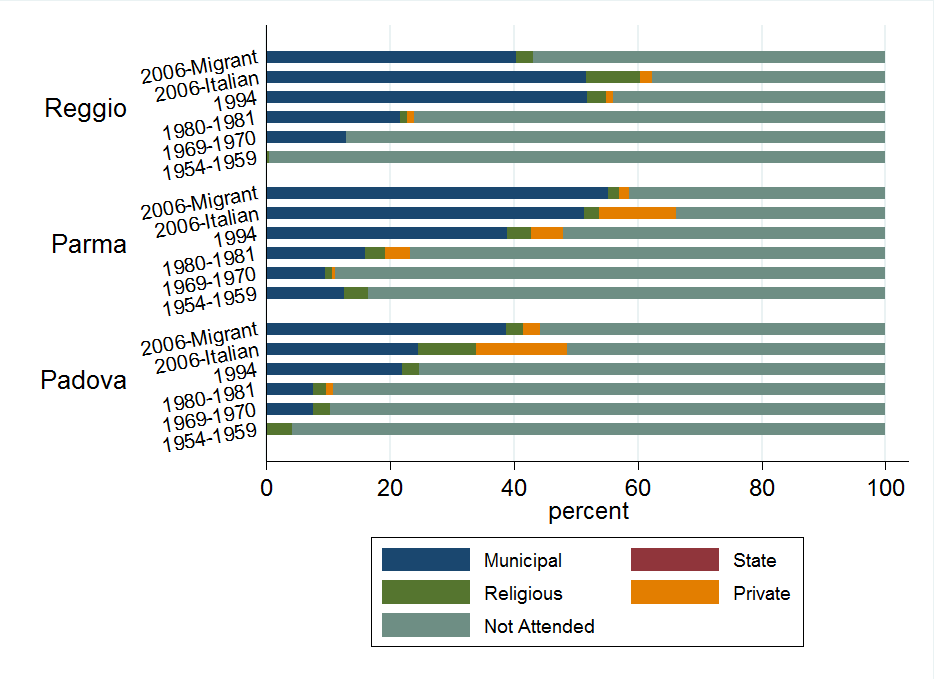
\includegraphics[scale=0.4]{../../../../output/image/asiloType-Attend.png} 
\end{figure}

\begin{figure}[H]
\caption{Type of Preschool Attended, by City and Cohort} \label{fig:attended-preschool}
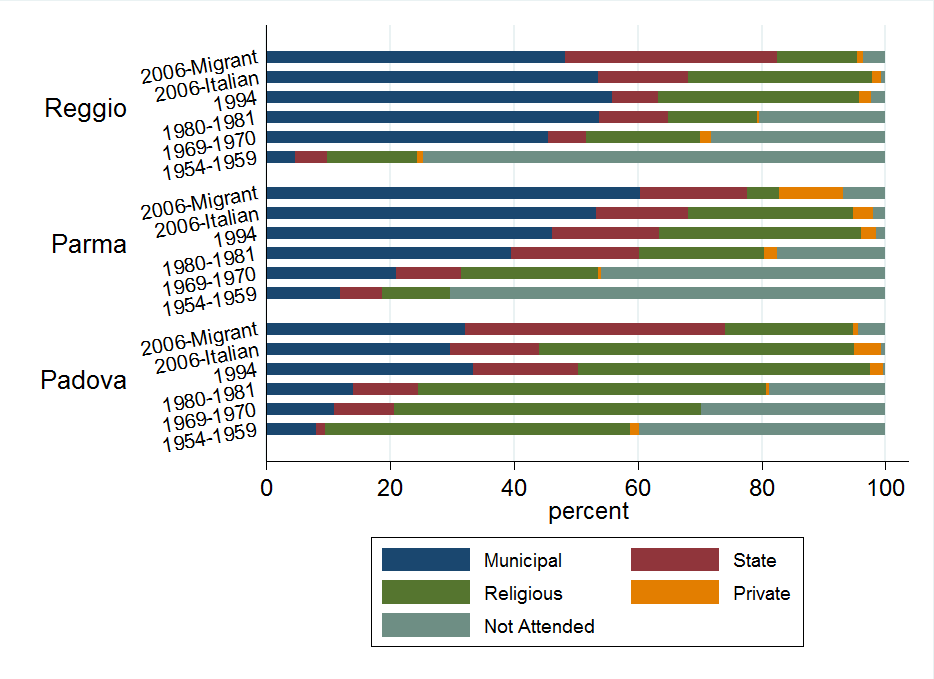
\includegraphics[scale=0.4]{../../../../output/image/maternaType-Attend.png} 
\end{figure}


\section{Parma}
\subsection{Asilo}

According to our current evidence, the first municipal infant-toddler centers in Parma were likely to be opened in 1975 after the National Law. However, according to Figure \ref{fig:attended-itc} people who were born between 1954-1959 and between 1969-1970 reported that they attended municipal infant-toddler centers in Parma. Since this information from the data is not consistent with the historical fact, we look into self-reported information of those individuals. 

\begin{landscape}
\begin{table}[H] \caption{Self-Reported Municipal Asilo Information for Age-40 Cohort in Parma}
\scalebox{0.85}{
\begin{tabular}{L{1.7cm} L{5cm} L{2.8cm} L{4.2cm} L{4.2cm} L{2.5cm} L{3.5cm}}
\toprule
\textbf{ID} & \textbf{Type*} & \textbf{School Name} & \textbf{School Address} & \textbf{Assigned School*} & \textbf{Accuracy*} & \textbf{Date Founded*} \\ \midrule
51088600 & Municipal & N/A & Stradello San Girolamo & Acquerello & 0.8 & Unknown \\
51051900 & Municipal-Parmainfanzia   & Nido D'Infanzia Aladino & San Prospero & Aladino & 0.9 & 2011 \\
51044100 & Municipal-Parmainfanzia   & N/A & Via La Grola & Bolle Di Sapone & 0.5 & Unknown \\
53009900 & Municipal-Parmainfanzia   & N/A & Prati Bocchi & Bolle Di Sapone & 0.5 & Unknown \\
54245100 & Municipal-Parmainfanzia   & N/A & Prati Bocchi & Bolle Di Sapone & 0.5 & Unknown \\
51048200 & Municipal			     & N/A & Via Pini & Ficco Di Neve & 0.8 & Unknown \\
51051200 & Municipal-Parmainfanzia   & Girotondo & N/A & Girotondo & 0.8 & Unknown \\
51051800 & Municipal-Parmainfanzia   & Nido D'Infanzia Comunale Girotondo & Via San Donato & Girotondo & 0.8 & Unknown \\
51088800 & Municipal-Parmainfanzia   & N/A & San Donato  & Girotondo & 0.9 & Unknown \\
51050900 & Municipal-Parmainfanzia   & N/A & Strada Constituente & Trottola & 0.6 & 2005 \\
54245600 & Municipal-Parmainfanzia   & N/A & San Lazzaro & Mappamondo & 0.6 & Unknown \\
51045600 & Municipal			     & N/A & Fognano & Primavera & 0.8 & 2003 \\
51045700 & Municipal			     & N/A & Fognano & Primavera & 0.8 & 2003 \\
51045800 & Municipal			     & N/A & Fognano & Primavera & 0.8 & 2003 \\
53007000 & Municipal			     & N/A & Fognano & Primavera & 0.8 & 2003 \\
53007100 & Municipal			     & N/A & Fognano & Primavera & 0.8 & 2003 \\
53011500 & Municipal			     & N/A & San Pancrazio  & Primavera & 0.1 & 2003 \\
53011600 & Municipal			     & N/A & San Pancrazio  & Primavera & 0.1 & 2003 \\
51055500 & Municipal			     & Zucchero Filato & Via Torrente Pessola & Zucchero Filato & 1 & Unknown \\
51053900 & Religious-FISM-affiliated & Nido D'Infanzia Casa Famiglia E Picco & Via Cocconcelli & Eugenia & 1 \\
51044500 & Religious-FISM-affiliated & San Benedetto & Via S,Benedetto & Ausiliatrice & 0.8 & 1891 \\
51052500 & Municipal-Affiliated		 & Asilo Nido Lilliput & Via Moletolo & Lilliput & 1 & 2005 \\
\bottomrule
\end{tabular}}
\end{table}

\begin{table}[H] \caption{Self-Reported Municipal Asilo Information for Age-50 Cohort in Parma}
\scalebox{0.85}{
\begin{tabular}{L{1.7cm} L{5cm} L{2.8cm} L{4.2cm} L{4.2cm} L{2.8cm} L{3.5cm}}
\toprule
\textbf{ID} & \textbf{Type*} & \textbf{School Name} & \textbf{School Address} & \textbf{Assigned School*} & \textbf{Accuracy*} & \textbf{Date Founded*}  \\ \midrule
51047600 & Municipal					& N/A 	& 	Vigatto			& Arcobaleno  & 0.4	& 2000 \\
51049800 & Municipal-Parmainfanzia		& N/A 	&	Prati Bocchi	& Bolle Di Sapone & 0.5 & Unknown \\
53004700 & Municipal					& N/A 	&	Fognano			& Primavera  & 0.8 & 2003	\\
53004800 & Municipal					& N/A 	&	Fognano			& Primavera  & 0.8 & 2003	\\
51043600 & Religious-FISM-Affiliated	& Orsoline 	&	Corpus Domini & Corpus Domini & 1	& 1961 \\
51050500 & Religious-FISM-Affiliated	& N/A 	&	Crocetta		& Marchi & 0.7	& 1972	\\
52980000 & Religious-FISM-Affiliated	& Parrocchiale Di Vigatto 	&	Via Martinella, Vigatto & Assunta	 & 0.8 & Unknown	\\
51044800 & Municipal-Affiliated			& N/A 	&	Baganzola & Cornocchio & 0.9 & Unknown 	\\
51045000 & Municipal-Affiliated			& N/A 	&	Baganzola & Cornocchio & 0.9 & Unknown	\\
51045100 & Municipal-Affiliated			& N/A 	&	Baganzola & Cornocchio & 0.9 & Unknown	\\
51045300 & Municipal-Affiliated			& N/A 	&	Baganzola & Cornocchio & 0.9 & Unknown	\\
\bottomrule
\end{tabular}}
\end{table}
\end{landscape}



\end{document}